- datasets

-- unimorph

-- bibles corpus?

-- celex


- permute phonemes

- permute syllables

- permute phonemes only within syllables

- permute morphemes 

\section{Morphology}

Bybee 1985:

verb-valence-voice-aspect-tense-mood-modality-subj.person-subj.number

can also directly quantify MI with verb stem (presence \& choice for each slot) as a sanity check

We study two agglutinative languages for which extensive corpora with hand-annotated morphological segmentation and labeling is available.

\subsection{Japanese Verb Suffixes}


\paragraph{Data Selection and Processing}
We drew on Universal Dependencies data.
In the tokenization scheme used for Japanese, most affixes are separated as individual tokens, effectively providing morpheme segmentations.
We used the GSD corpus, Version 2.4, \citep{tanaka2016universal, asahara2018universal}, as it was the only corpus with a training set and freely available word forms.

In the corpus, verb suffixes largely correspond to auxiliaries (tag AUX); only a few morphemes tagged AUX are not standardly treated as suffixes (see SI), and one frequent suffix (-\textit{te}) is labeled SCONJ.

We selected verb forms by selecting all chains of a verb (tag VERB) followed by any number of auxiliaries (tag AUX) from the training set of the corpus. When the suffix -\textit{te} (tag SCONJ) followed such a chain, we added this.

We obtained 15,281 verb forms, with a median number of X suffixes (max=...).

In the corpus, each morpheme is annotated with a lemma, indicating a normalized context-independent representation of the morpheme.
For both verbs and affixes, this lemma annotation abstracts away from most morphophonological and other allomorphic variation, it thus largely identifies underlying morphemes (see SI for limitations).


\paragraph{Verb Suffixes in Japanese}

Japanese has an extensive number of suffixes, including rarer ones that are not well represented in the corpus.
Based on the corpus and the linguistic literature on Japanese, we identified the following frequent verb suffixes, occurring in the following order outwards from the verb (see SI for details).


\begin{enumerate}
\item Valence: causative (-\textit{ase}-) (\citet[142]{hasegawa2014japanese}, \citet[Chapter 13]{kaiser2013japanese})
\item Voice: passive (-\textit{are}-, -\textit{rare}-) \cite[152]{hasegawa2014japanese} \cite[Chapter 12]{kaiser2013japanese}
\item Mood: potential (-\textit{e}-, -\textit{are}-, -\textit{rare}-)  
\item politeness (-\textit{mas}-) \cite[190]{kaiser2013japanese}.
\item Mood: desiderative (-\textit{ta}-) \cite[238]{kaiser2013japanese}
\item Negation (-\textit{n}-)
\item Tense/Aspect/Mood: past (-\textit{ta}) and future/hortative (-\textit{yoo}) \cite[229]{kaiser2013japanese}
\item Nonfiniteness: the suffix -\textit{te} derives a nonfinite form \cite[186]{kaiser2013japanese}.
\end{enumerate}

In accordance with Bybee's hierarchy, valence is marked closest to the verb, followed by voice.
Unlike predicted by the hierarchy, tense/aspect markers are not placed closer to the verb than mood/modality markers.



\paragraph{Experiment}

modes:

We considered three methods of quantifying prediction
(1) on the level of phonemes, (2) on the level of graphemes, (3) on the level of morphemes.

For (1): Many verb stems are written using Kanji characters; we did not phonemize these. (TODO probably we should do this to make things clean).


For (3), we label suffixes for underlying morphemes with the aid of provided lemmatization (see SI for details)
This controls for allomorphy / morphophonemic changes, which are conditioned on surrounding affixes.
By conducting these 

\paragraph{Parameterizing Alternative Orderings}

We parameterize alternative suffix orderings by assigning an integer to each morpheme.
We consider all morphemes annotated in the corpus, including those less frequent than the ones identified above (see SI for details).

\paragraph{Creating Optimal Orders}

We optimize orderings for the AUC under the memory-surprisal tradeoff curve with an adaptation of the hill climbing method used by (CITE) to optimize word order grammars for the length of syntactic dependencies.

We randomly initialize the assignment of integers to morphemes.

In each iteration, we randomly choose one morpheme, and evaluate AUC for each way of ordering it between two other morphemes.
We then update the weights to the ordering that yields the lowest AUC.

Computation of AUC is approximated at $T=5$ for computational efficiency.

To further speed up optimization, we restrict to morphemes occurring at least 10 times in the corpus for about 95\% of iterations, and to about 10\% of possible orderings in each step.
These choices vastly reduce computation time by reducing time spent on low-frequency morphemes.

We run this for X iterations.

\paragraph{Results: Comparison to Baselines}
comparison to baselines

- random grammars


\begin{figure}
	\begin{center}
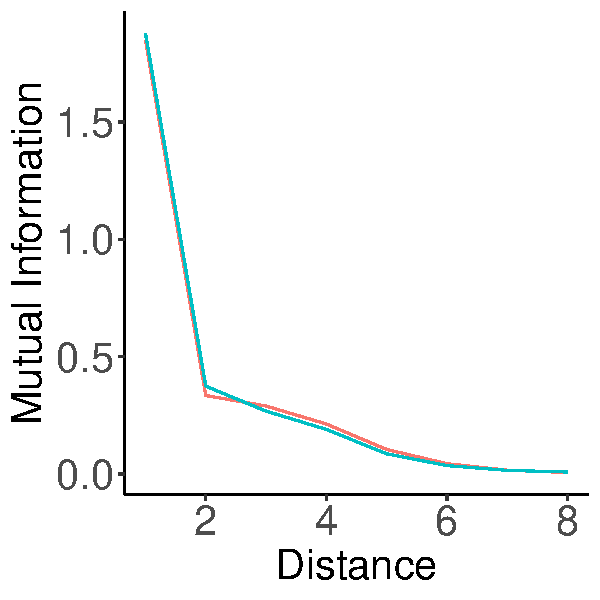
\includegraphics[width=0.3\textwidth]{figures/Japanese-suffixes-byPhonemes-it.pdf}
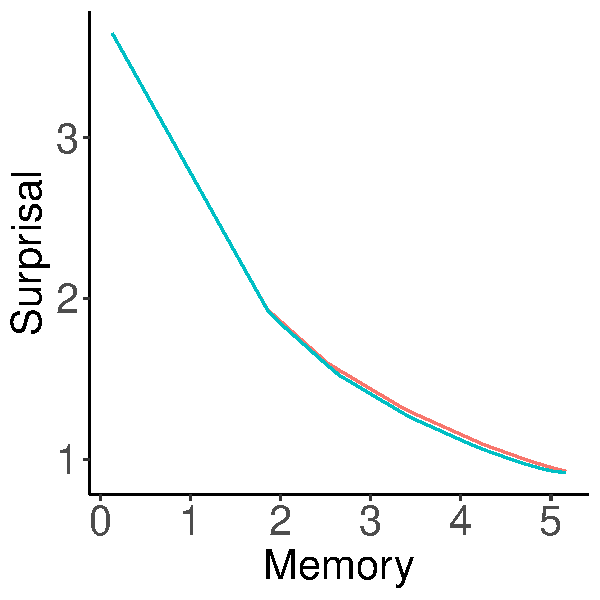
\includegraphics[width=0.3\textwidth]{figures/Japanese-suffixes-byPhonemes-memsurp.pdf}

\includegraphics[width=0.3\textwidth]{figures/Japanese-suffixes-byPhonemes-auc.pdf}
\end{center}
	\caption{Japanese verb suffixes, measuring prediction on the level of phonemes, for real (blue), random (green), and optimized (red) orderings. Left: $I_t$ as a function of $t$. Center: Memory-surprisal tradeoff. Right: Areas under the curve for the memory-surprisal tradeoff.}\label{fig:jap-phon}
\end{figure}


\begin{figure}
	\begin{center}
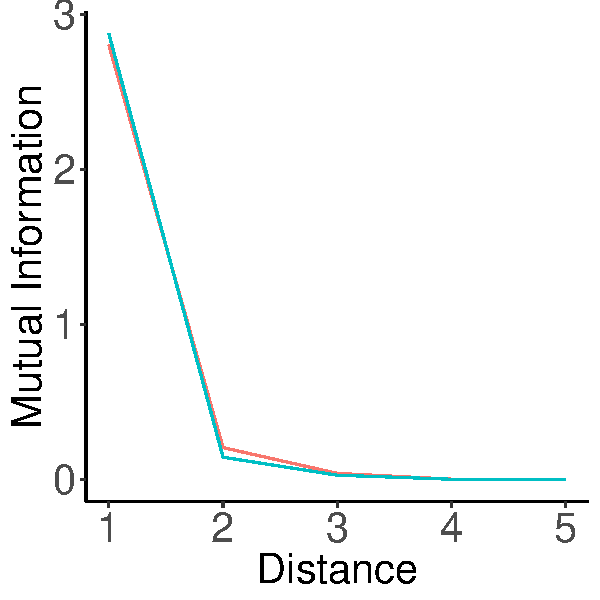
\includegraphics[width=0.3\textwidth]{figures/Japanese-suffixes-byMorphemes-it.pdf}
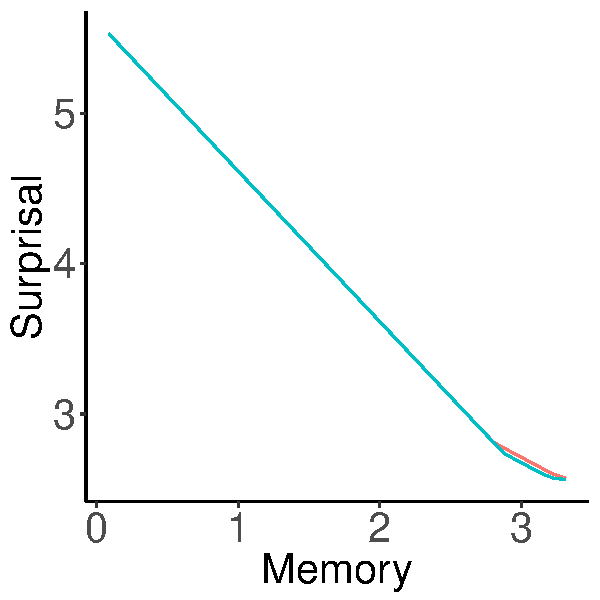
\includegraphics[width=0.3\textwidth]{figures/Japanese-suffixes-byMorphemes-memsurp.pdf}
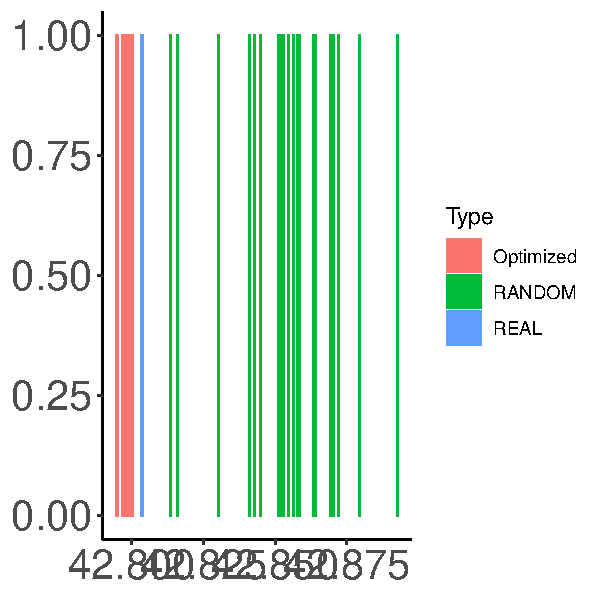
\includegraphics[width=0.3\textwidth]{figures/Japanese-suffixes-byMorphemes-auc.pdf}
\end{center}
	\caption{Japanese verb suffixes, measuring prediction on the level of morphemes, for real (blue), random (green), and optimized (red) orderings. Left: $I_t$ as a function of $t$. Center: Memory-surprisal tradeoff. Right: Areas under the curve for the memory-surprisal tradeoff.}\label{fig:jap-morph}
\end{figure}


\paragraph{Results: Comparing Optimized and Real Orders}

- phonemes

- graphemes

- morphemes


\begin{tabular}{c|ccccc}
             & Pair Accuracy & Full Accuracy \\ \hline
Phonemes     &   \\
Morphemes     &  \\
\end{tabular}



\subsection{Sesotho}

Sesotho (also known as Southern Sotho) is a Southern Bantu language, spoken by 5.6 Million L1 speakers (REF) mainly in Lesotho and South Africa.
We use the Demuth Corpus \citep{demuth1992acquisition} of child and child-directed speech, containing about 13K utterances with 500K morphemes.
The corpus has very extensive manual morphological segmentation and annotation; each verb form is segmented into morphemes, which are annotated for their function.

Sesotho verbs carry both prefixes and suffixes.
We extracted 37K verb forms (see SI for details).


\paragraph{Verb Affixes in Sesotho}

We identified morphemes and morpheme ordering based on the analysis in \cite{demuth1992acquisition}, supplemented with information from grammars of Sesotho \citep{doke1967textbook,guma1971outline}. See SI for details.

Prefixes:

\begin{enumerate}
    \item Subject agreement: This morpheme encodes agreement with the subject, for person, number, and noun class (the latter only in the 3rd person) \cite[\textsection 395]{doke1967textbook}.
    
    \item Negation 
    
    \item Tense/aspect marker  Guma 1971, p. 165-166. \cite[\textsection 400-424]{doke1967textbook}
    
    \item Object agreement or reflexive marker. 
    Similar to subject agreement, object agreement denotes person, number, and noun class features of the object.
    Unlike subject agreement, it is optional (CITE).
    \end{enumerate}
    
    Suffixes:
    
    \begin{enumerate}
    \item Valence: causative (-isa),  neuter/stative (-eha, -ahala), applicative (-el-), reciprocal (-an-)
    
    
    Also two that aren't really valence:
    
    - reversive \cite[\textsection 345]{doke1967textbook} -- not really VALENCE, ex. bind -- loosen
    
    -  Perfective/Completive (-ets), -ell (66 times) \cite[\textsection 336]{doke1967textbook}
    

    \item Voice: passive (-iw-)
    
    
    \item Tense: The only tense suffix is the perfect affix -il-.

     
    \item MOOD: Mood (m\^{}, 37K times), such as -a/-e for indicative \citep{demuth1992acquisition}.
    

    \item Interrogative (labeled \textit{wh}, 2K times) and relative (labeled \textit{rl}, 857 times) markers -\textit{ng}
    
    The interrogative eng `what' can be encliticized to the verb; this is treated as a suffix in the Demuth corpus \cite[p. 168]{guma1971handbook}, \cite[\textsection 160, 320]{doke1967textbook}.
    
    Verbs in relative clauses are marked with -ng \cite[\textsection 271, 793]{doke1967textbook}

\end{enumerate}



For prefixes, in agreement with Bybee's hierarchy, subject agreement is encoded in a position further away than TAM features.

For suffixes,
relation to Bybee hierarchy: valence closest, then voice, then tense, then mood.




\paragraph{Experiment}

modes:

We considered three methods of quantifying prediction
(1) on the level of phonemes, (2) on the level of graphemes, (3) on the level of morphemes.

For (1): Many verb stems are written using Kanji characters; we did not phonemize these. (TODO probably we should do this to make things clean).


For (3), we label suffixes for underlying morphemes with the aid of provided lemmatization (see SI for details)
This controls for allomorphy / morphophonemic changes, which are conditioned on surrounding affixes.
By conducting these 

\paragraph{Parameterizing Alternative Orderings}

We parameterize alternative suffix orderings by assigning an integer to each morpheme.
We consider all morphemes annotated in the corpus, including those less frequent than the ones identified above (see SI for details).

\paragraph{Creating Optimal Orders}

\paragraph{Results: Comparison to Baselines}
comparison to baselines

- random grammars



\begin{figure}
	\begin{center}
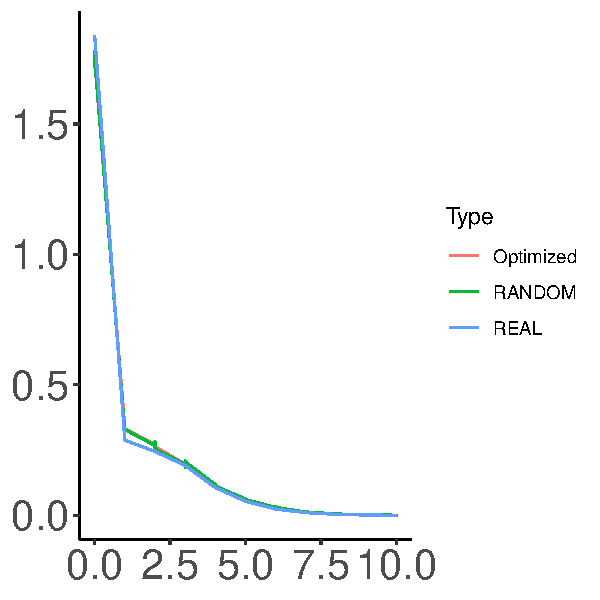
\includegraphics[width=0.3\textwidth]{figures/Sesotho-suffixes-byPhonemes-it.pdf}
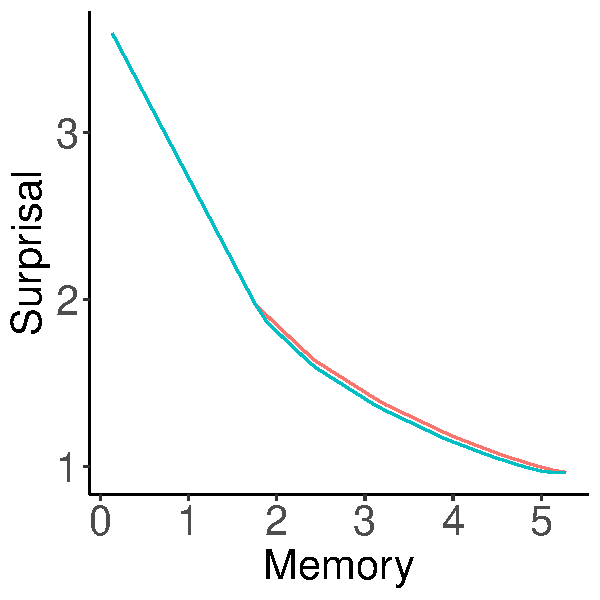
\includegraphics[width=0.3\textwidth]{figures/Sesotho-suffixes-byPhonemes-memsurp.pdf}
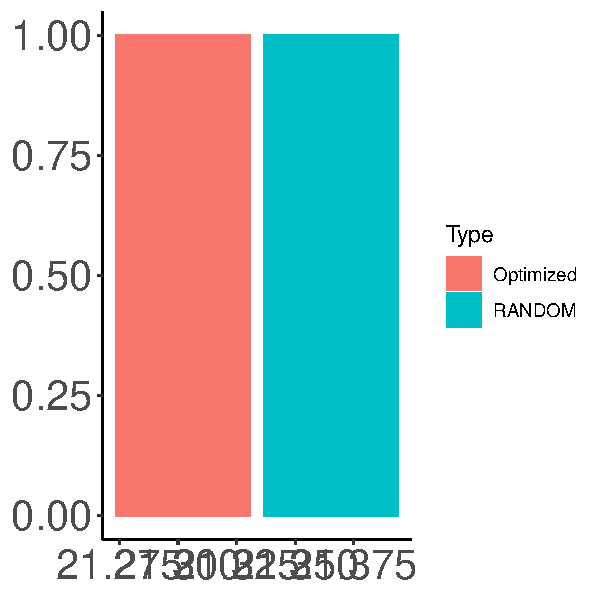
\includegraphics[width=0.3\textwidth]{figures/Sesotho-suffixes-byPhonemes-auc.pdf}
\end{center}
	\caption{Sesotho verb suffixes, measuring prediction on the level of phonemes, for real (blue), random (green), and optimized (red) orderings. Left: $I_t$ as a function of $t$. Center: Memory-surprisal tradeoff. Right: Areas under the curve for the memory-surprisal tradeoff.}\label{fig:jap-phon}
\end{figure}


\begin{figure}
	\begin{center}
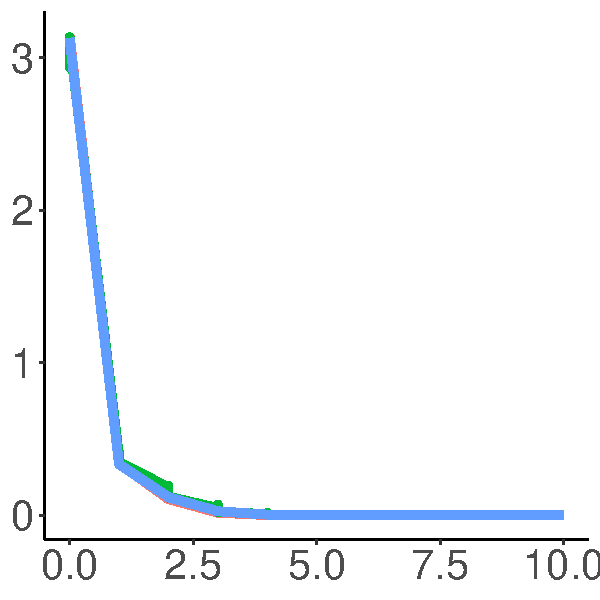
\includegraphics[width=0.3\textwidth]{figures/Sesotho-suffixes-byMorphemes-it.pdf}
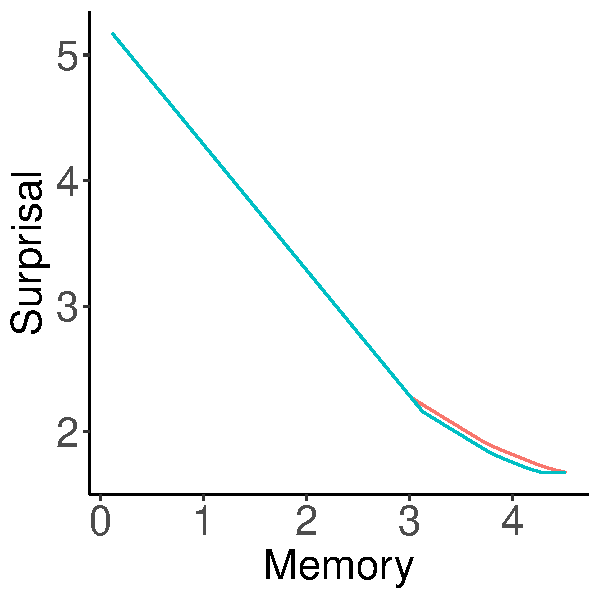
\includegraphics[width=0.3\textwidth]{figures/Sesotho-suffixes-byMorphemes-memsurp.pdf}
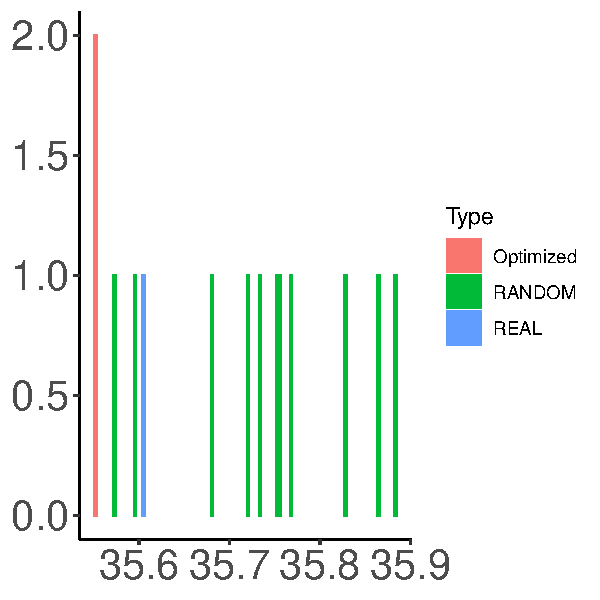
\includegraphics[width=0.3\textwidth]{figures/Sesotho-suffixes-byMorphemes-auc.pdf}
\end{center}
	\caption{Sesotho verb suffixes, measuring prediction on the level of morphemes, for real (blue), random (green), and optimized (red) orderings. Left: $I_t$ as a function of $t$. Center: Memory-surprisal tradeoff. Right: Areas under the curve for the memory-surprisal tradeoff.}\label{fig:jap-morph}
\end{figure}


\paragraph{Results: Comparing Optimized and Real Orders}

- phonemes

- graphemes

- morphemes

